\chapter[Otimização multiobjetivo]{Otimização multiobjetivo}

A otimização multiobjetivo consiste em selecionar as melhores soluções de acordo com múltiplos critérios. Por exemplo, ao estabelecer o melhor caminho entre duas cidades pode-se não estar interessado apenas na menor distância, mas também no tráfego, segurança das vias, quantidade de pedágios, etc. Na otimização com um único objetivo, a comparação entre soluções é relativamente simples. Para que uma solução seja considerada melhor que a outra, basta que ela tenha uma melhor avaliação segundo o critério/métrica considerada. Por outro lado, quando se trabalha com mais de uma função de otimização, é preciso adotar alguma estratégia mais elaborada. Por exemplo, pode ser possível aplicar algum tipo de ponderação entre os valores dos diferentes objetivos, combinando-se as funções em um único objetivo. De forma alternativa, existem diversas abordagens que mantêm os objetivos separados e trabalham com o conceito de dominância de Pareto, como os algoritmos NSGA-II \cite{Deb2002} e SPEA2 \cite{Zitzler2002}.

A dominância de Pareto estabelece que uma solução $A$ é melhor que uma solução $B$, ou $A$ domina $B$ ($A \prec B$), se, e somente se:

\begin{itemize}  
	\item $A$ é melhor avaliado que $B$ em pelo menos um dos objetivos;
	\item $A$ não tem avaliação pior que $B$ em nenhum dos objetivos.
\end{itemize}

Considerando-se um problema de minimização e $F$ como o conjunto de funções objetivo, tem-se, matematicamente:

\begin{equation}A \prec B \Leftrightarrow (\forall(f \in F) f(A) \leq f(B)) \land (\exists (f \in F) f(A) < f(B))\end{equation}

Em problemas de otimização multiobjetivo, geralmente o objetivo está em encontrar o conjunto Pareto ótimo, ou seja, o conjunto de todas as soluções do espaço de busca que não são dominadas por nenhuma outra e cujo mapeamento para o espaço de objetivos forma a Fronteira de Pareto. Graficamente, a fronteira de Pareto representa a linha formada pelas soluções não-dominadas existentes para o problema. Na \autoref{fig_pareto} apresenta-se um exemplo da fronteira de Pareto para um problema de minimização com dois objetivos ($F1$ e $F2$). Nesse exemplo, os pontos pertencentes à fronteira de Pareto estão destacados em vermelho. Observe que, todas as soluções pertencentes à fronteira de Pareto são não dominadas, ou seja, nenhum ponto da fronteira possui ambos valores menores que alguma outra solução em ambas as funções ($F1$ e $F2$). Em contrapartida, toda solução acima da fronteira (pontos em cinza) é dominada, pois existe alguma solução em vermelho que possui ambos valores de F1 e F2 menores.

\begin{figure}
	\centering
	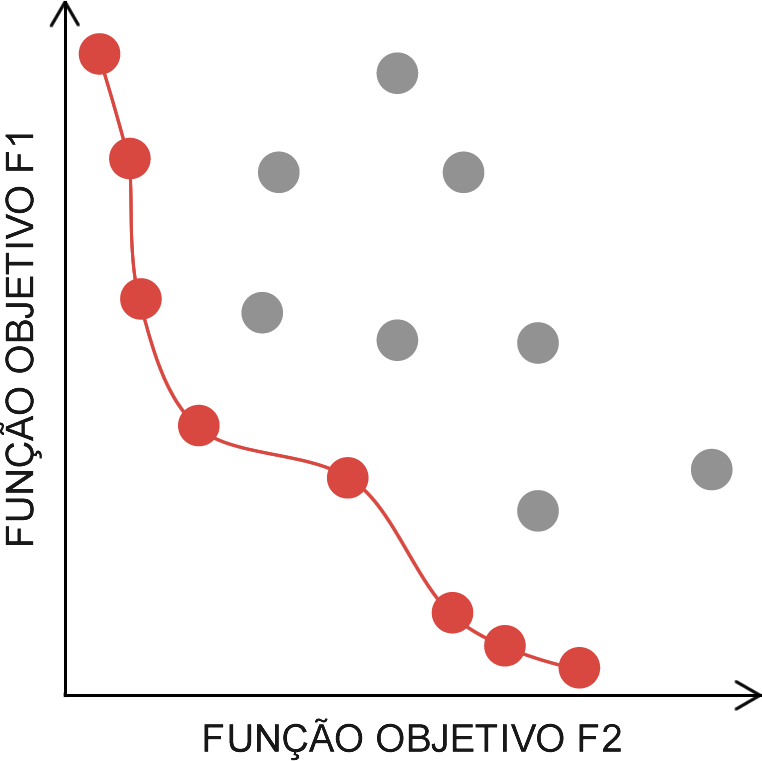
\includegraphics[width=0.4\textwidth]{cap_otimizacao-multi/figs/pareto}
	\caption{\label{fig_pareto}Fronteira de Pareto}
\end{figure}

Não existe limite para o número de funções objetivo em um problema de otimização, mas quanto maior a quantidade de objetivos, mais complexa é a busca \cite{Deb2014}. Os algoritmos clássicos de otimização multiobjetivo \ac{NSGA-II} e \ac{SPEA2} lidam bem com até três objetivos, mas a partir de quatro critérios de otimização, ambos os métodos sofrem para encontrar soluções que fazem parte do conjunto Pareto ótimo do problema. Desta forma, criou-se a classificação ``\textit{many-objective}''. Problemas \textit{many-objective} (4 ou mais objetivos) apresentam um maior grau de dificuldade e demandam novas técnicas para que sejam resolvidos eficientemente. Analisando as abordagens baseadas em algoritmos evolutivos multiobjetivos (AEMOs), \citeonline{Deb2014} observaram os seguintes os problemas trazidos pelo alto número de objetivos:

\begin{enumerate}  
	\item \textbf{Grande parte da população é não dominada:} a maioria dos algoritmos multiobjetivos classifica a população de acordo com a dominância de Pareto. Se existem muitas funções objetivo, é muito comum que uma solução seja melhor que outra em pelo menos uma delas. Desta forma, a maior parte das soluções se torna não-dominada, o que impede os algoritmos de evoluírem a população, já que todos os indivíduos são considerados igualmente bons.
	\item \textbf{Avaliar a diversidade da população se torna computacionalmente caro:} a fim de garantir uma boa diversidade populacional, os algoritmos adotam alguma medida de distância entre as soluções e removem aquelas consideradas mais similares. O aumento na dimensionalidade traz consequentemente um maior impacto (complexidade e custo) no cálculo da proximidade entre os indivíduos. 
	\item \textbf{\textit{Crossover} ineficiente:} a alta dimensionalidade do espaço de busca faz com que os indivíduos na população sejam muito distantes uns dos outros e, normalmente, o cruzamento entre duas soluções muito diferentes resultam num filho muito distante dos pais, o que prejudica a convergência da busca. Portanto, pode ser necessário redefinir os operadores de recombinação a fim de restringir as possibilidades de pareamento.
	\item \textbf{População demasiadamente grande:} quanto maior o número de objetivos, maior o número de soluções na fronteira de Pareto. Portanto, para se obter bons resultados, é necessário que se manipule grandes populações de indivíduos, o que é computacionalmente caro e dificulta a análise do usuário que deverá escolher uma única solução ao final do processo.
	\item \textbf{Métricas de análise de desempenho do algoritmo se tornam difíceis de calcular:} a avaliação do resultado do algoritmo (taxa de erro, distância para o Pareto, hiper-volume, etc.) está diretamente relacionada ao número de objetivos. Quanto maior ele for, maior será o esforço computacional necessário. A complexidade do hiper-volume, por exemplo, cresce exponencialmente com o número de objetivos.
	\item \textbf{Dificuldade de visualização:} é fácil representar graficamente as soluções e a fronteira de Pareto em problemas de até três objetivos. Entretanto, não existe uma forma eficiente de visualizar os resultados para problemas que lidam com maior dimensionalidade (4 objetivos em diante).
\end{enumerate}

A maior parte dos algoritmos \textit{many-objectives} mencionados neste trabalho buscam lidar com os quatro primeiros problemas. As duas últimas não se relacionam diretamente aos algoritmos de otimização em si, mas sim à análise da qualidade das soluções encontradas.

\section{Algoritmos Bio-Inspirados Multiobjetivos}
\label{section_bioinspired_algorithms}

A maior parte dos métodos de busca multiobjetivo é baseada em algoritmos inspirados na biologia. Esses algoritmos são adaptações das estratégias evolutivas, colônias de formigas e enxames de partículas tradicionais para lidar com problemas que envolvam mais de um objetivo. A principal diferença entre um algoritmo de otimização tradicional e sua variação multiobjetivo está na forma de cálculo da aptidão dos indivíduos da população. No caso dos algoritmos multiobjetivos, geralmente o conceito de dominância é usado de diferentes formas \cite{Bueno2010}.

A seguir são apresentados alguns algoritmos bio-inspirados multiobjetivo encontrados na literatura. Os dois primeiros (NSGA-II e SPEA2) são algoritmos bem conhecidos e largamente utilizados em problemas multiobjetivos. Apesar de sua eficiência na resolução de problemas com até 3 objetivos, o desempenho desses AEMOs costuma cair consideravelmente com o aumento no número de objetivos \cite{Franca2017}. Os demais algoritmos apresentados, são mais recentes e foram concebidos especificamente para tratar de problemas \textit{many-objective}, ou seja, que envolvam 4 ou mais objetivos.

\subsection{NSGA-II}
O \textit{Non-dominated Sorting Genetic Algorithm II} (NSGA-II) \cite{Deb2002} é o algoritmo evolutivo multiobjetivo mais frequente na literatura. O processo desse algoritmo é semelhante ao do algoritmo genético comum, com diferença no cálculo de aptidão, que é feito por \textit{ranks}, e no cálculo de distâncias, que é inexistente na proposta original do AG. A atribuição de aptidão (\textit{fitness}) se dá pela classificação da população em categorias/classes (\textit{rankings}) de dominância (fronteiras), de forma que o primeiro contenha todas as soluções não dominadas, o segundo todos os indivíduos não-dominados excluindo aqueles presentes na primeira fronteira, e assim por diante. Quanto melhor o \textit{ranking} de uma solução, melhor sua aptidão e  maior sua chance de sobreviver para a próxima geração. Várias soluções podem pertencer a uma mesma fronteira. A fim de diferenciá-las entre si, é utilizado um cálculo de distância (\textit{crowding distance}), o qual confere melhor avaliação às soluções mais esparsas de uma mesma fronteira (maior distância em relação às outras soluções da fronteira), garantindo assim a diversidade da população.

O fluxo de funcionamento do NSGA-II inicia-se com a geração aleatória dos indivíduos. Em seguida, a população é classificada em fronteiras de dominância (ou \textit{ranks}) e inicia-se o processo iterativo, o qual termina assim que a condição de parada é atingida. As etapas que compõem cada iteração do NSGA-II são descritas no pseudo-código do algoritmo \ref{alg_nsgaii}.

\begin{algorithm}
	\caption{Processo iterativo do NSGA-II}
	\label{alg_nsgaii}
	\begin{algorithmic}[1]
		\While {critério de parada não for atingido}
		\State $Pais \gets selecao(Pop_{atual}, TX_{cross})$
		\State $Filhos \gets crossover(Pais)$
		\State $Pop_{nova} \gets Pop_{atual} \cup Filhos$
		\State $ranks \gets ranking(P_{nova})$
		\State $crowdingDistance(P_{nova})$
		\State $Pop_{atual} \gets reinsercao(ranks, tam_{populacao})$
		\EndWhile
	\end{algorithmic}
\end{algorithm}

O processo iterativo do algoritmo inicia-se com a seleção dos pares de pais para o cruzamento (linha 2). Na implementação considerada, a seleção de pais utiliza torneio simples com \textit{tour} de 2, ou seja, dois elementos da população são escolhidos de forma aleatória e o indivíduo com melhor avaliação é selecionado como um dos pais. Então, esse processo é repetido para a escolha do segundo pai.

Na linha 3 do pseudo-código, através dos pares de pais, geram-se os filhos com o \textit{crossover} e a mutação. Após a geração dos filhos, a população corrente e o conjunto de filhos são concatenados (linha 4) e submetidos à classificação em fronteiras de dominância (\textit{ranks}) na linha 5).

A classificação em fronteiras de dominância recebe um conjunto de soluções e verifica quais dentre elas não são dominadas. O conjunto de soluções não-dominadas forma a primeira fronteira de dominância. Do conjunto restante (excluindo a primeira fronteira), retiram-se as soluções não dominadas para formar a segunda fronteira. Esse processo se repete até que todos os indivíduos tenham sido classificados.

Após toda a população ter sido classificada em fronteiras, na linha 6, o algoritmo calcula a distância de aglomeração (\textit{crowding distance}) dos indivíduos em cada fronteira de dominância. O cálculo da distância, considerando cada objetivo avaliado, ordena o conjunto de soluções e faz uma relação entre as distâncias de cada indivíduo para os vizinhos adjacentes (que estão imediatamente antes ou depois). A distância de aglomeração de cada indivíduo é resultado da somatória das distâncias resultantes em cada objetivo.  Quanto maior o valor, maior é a diferença entre o indivíduo e seus pares dentro do \textit{rank}. Essa métrica é usada para manter a diversidade das soluções entre as gerações do algoritmo.

Com toda a população classificada em fronteiras (ou \textit{ranks}) e todas as distâncias calculadas, na linha 7, uma nova população é escolhida com base nos melhores indivíduos entre pais e filhos. Para isso, analisa-se fronteira a fronteira, da melhor para a pior, até que o tamanho máximo da população seja atingido. Para cada fronteira aplica-se o seguinte processo de decisão:

\begin{itemize}  
	\item Se $tamanho(fronteira) + tamanho(novaPopulação) < tamPop$: adicionam-se todos os membros da fronteira à nova população.
	\item Caso contrário: adicionam-se à nova população os ($tamPop - tamanho(novaPopulação)$) elementos da fronteira com os maiores valores de distância.
\end{itemize}

Desta forma, ao final do algoritmo obtém-se a fronteira de Pareto aproximada na primeira fronteira da população gerada na última iteração do algoritmo.

\subsection{SPEA2}

O \textit{Strength Pareto evolutionary algorithm 2} (SPEA2) \cite{Zitzler2002} é um AEMO que calcula, para cada membro da população, sua força (\textit{strength}) e densidade. A força de uma solução é dada pelo número de indivíduos que ela domina, enquanto a densidade é uma medida de distância para os vizinhos mais próximos, quanto maior a densidade mais próximo o indivíduo está das demais soluções. A aptidão (\textit{fitness}) de uma solução é definida por sua densidade mais a soma das forças de todo indivíduo que a domina. 

Os indivíduos mais aptos no SPEA2 são aqueles dominados pela menor quantidade de soluções e que possuem maior variabilidade genética. O algoritmo calcula a aptidão em três etapas: cálculo de força (\textit{strength}), da aptidão crua (\textit{raw fitness}) e da densidade \cite{Zitzler2002}.

A força de um indivíduo $i$ ($s(i)$) é o número de soluções que ele domina, ou seja, considerando $A$ o arquivo e $P$ a população:

\begin{equation}s(i) = |j|: j \in P \cup A \land i \prec j\end{equation}

Uma vez calculada a força de cada indivíduo, parte-se para o cálculo do \textit{raw fitness}. O \textit{raw fitness} de um indivíduo $i$ ($r(i)$) é dado pela soma das forças de cada elemento que o domina, como segue:

\begin{equation}r(i) = \sum_{j \in A \cup P | j \prec i} s(j)\end{equation}

Observe que, caso o indivíduo seja não-dominado, seu \textit{raw fitness} será o menor possível (zero). Para finalizar o cálculo de aptidão, é definida a densidade de cada indivíduo ($d(i)$). Essa densidade é computada de acordo com a distância da solução para seus vizinhos e é dada por:

\begin{equation}d(i) = \frac{1}{\sigma_i^k + 2}\end{equation}

Sendo, $\sigma_i^k$ a $k$-ésima menor distância entre o indivíduo $i$ e o restante da população; e $k$ a raiz quadrada do tamanho do conjunto de soluções em avaliação, i.e. $k = \sqrt{|P \cup A|}$. O valor de $d(i)$ sempre está no intervalo (0,1).

Finalmente, a aptidão do indivíduo ($f(i)$) é dada pela soma do \textit{raw fitness} e a densidade: 
\begin{equation}f(i) = r(i) + d(i)\end{equation}

Note que, se a solução $i$ é não-dominada, $f(i) < 1$. Isso ocorre dado que $d(i) < 1$ para qualquer solução e, quando $i$ é não-dominada, $r(i) = 0$.


Além do cálculo de aptidão, outra diferença importante entre o SPEA2 e um AG tradicional é a utilização de uma população extra, denominada arquivo. O arquivo é responsável por guardar as melhores soluções já encontradas até o momento, funciona como uma espécie de elitismo. Na seleção para o cruzamento, os pais são sempre escolhidos do arquivo e os filhos substituem 100\% da população corrente. A cada iteração, os melhores indivíduos entre a população e o arquivo compõem o arquivo da geração seguinte. A quantidade de indivíduos no repositório de soluções não-dominadas é limitada e, quando esse tamanho máximo ($tam_{arq}$) é excedido, deve-se executar um processo de truncamento.

O processo de truncamento de um arquivo ocorre na seleção natural (reinserção), que é a última função executada na iteração do laço principal de um AG. No SPEA2, a reinserção consiste em definir o arquivo para a próxima geração a partir das populações. Nesse processo, extraem-se do conjunto total de soluções (população e arquivo) aquelas que não são dominadas por nenhuma outra, e com esse subconjunto ($n_d$) constrói-se o novo arquivo através do seguinte processo de decisão:

\begin{itemize}  
	\item Se $tamanho(n_d) = tam_{arq}$, o novo arquivo é formado por $n_d$;
	\item Se $tamanho(n_d) < tam_{arq}$, o novo arquivo é formado pela união de $n_d$ com os $tam_{arq} - tamanho(n_d)$ indivíduos restantes com melhor aptidão;
	\item Caso contrário, ($tamanho(n_d) > tam_{arq}$), o novo arquivo é formado por $n_d$ e deve-se truncá-lo em ($tamanho(n_d) - tam_{arq}$) passos, onde em cada passo, elimina-se o indivíduo com menor variabilidade genética em relação aos demais.
\end{itemize}

O algoritmo retorna como resposta para o problema o arquivo resultante da última geração computada. Espera-se que, após as diversas iterações, o algoritmo tenha conseguido uma boa aproximação da fronteira de Pareto.

%O laço principal do SPEA2 é explicitado no algoritmo \ref{alg_spea2} e, como resposta para o problema, retorna-se o arquivo resultante da última geração computada. Espera-se que, após as diversas iterações, o algoritmo tenha conseguido uma boa aproximação da fronteira de Pareto.

%\begin{algorithm}
%	\caption{Laço principal do SPEA2}
%	\label{alg_spea2}
%	\begin{algorithmic}[1]
%		\While {número máximo de gerações não for atingido}
%		\State a partir do arquivo, selecione os pares de pais para o crossover
%		\State efetue o cruzamento para cada par de pais, gerando os filhos
%		\State substitua a população corrente pelos filhos
%		\State calcule o fitness de todos indivíduos no arquivo e na população
%		\State aplique a seleção natural e trunque o arquivo, caso necessário
%		\EndWhile
%	\end{algorithmic}
%\end{algorithm}

\subsection{MOEA/D}
\label{section_moead}

O \textit{Multiobjective evolutionary algorithm based on decomposition} (MOEA/D) \cite{Zhang2007} é um algoritmo que avalia os objetivos através de uma função escalarizadora, baseando-se na dominância de Pareto apenas para atualizar o conjunto de soluções não dominadas geradas em cada iteração. A esse conjunto, dá-se o nome de arquivo. No MOEA/D, um problema multiobjetivo é decomposto em múltiplos problemas de um único objetivo. Cada problema mono-objetivo é associado a uma célula da estrutura que armazena a população. Cada célula é definida por um vetor de pesos gerado aleatoriamente e representa um indivíduo, ou seja, o número de células é igual ao tamanho da população. Além dos pesos, a célula é composta de uma solução e uma vizinhança. A vizinhança é formada pelos $k$ indivíduos mais próximos de acordo com o vetor de pesos, onde $k$ é um parâmetro do algoritmo que representa o tamanho das vizinhanças. A aptidão (\textit{fitness}) de uma solução é calculada de acordo com sua avaliação em cada objetivo, a função escalarizadora, e o vetor de pesos da célula. Em toda geração, uma nova solução é gerada para cada célula, onde a vizinhança é considerada nas etapas de escolha dos pais e seleção natural.

O início do algoritmo consiste na geração da estrutura de células e na definição das vizinhanças. Para isso, sorteiam-se os vetores de pesos (a soma de cada vetor deve ser igual a um) e, para cada um deles, calculam-se os $k$ vetores mais próximos (vizinhança). Essa estrutura é imutável e é utilizada no decorrer de todo o algoritmo. A geração dos vetores de pesos pode ser tanto aleatória quanto seguir uma distribuição pré-definida (por exemplo, uma distribuição uniforme).

Uma parte fundamental do MOEA/D é a escolha da função escalarizadora, a qual é a principal responsável pelo cálculo de aptidão. Em todos experimentos realizados neste trabalho, foi utilizada a soma ponderada, mas outras estratégias, como \textit{Penalty-Based Boundary Intersection} (PBI) e decomposição de Tchebycheff também podem ser utilizadas \cite{Zhang2007}. A escolha da soma ponderada se baseou em experimentos preliminares que mostraram sua maior eficiência em relação à decomposição de Tchebycheff para os problemas avaliados. Além disso, é mostrado em \citeonline{ScalarizationFunctionsIshibuchi} que, para muitos objetivos, as funções de soma ponderada e PBI apresentam melhores resultados para o problema da mochila.

A aptidão de uma solução é calculada através da função escalarizadora e do vetor de pesos. Por exemplo, se os valores $[2; 9; 5]$ representam a solução $s$ no espaço de objetivos, $[0,3; 0,2; 0,5]$ é o vetor de pesos da célula $c$, e a soma ponderada é a função escalarizadora, então a aptidão de $s$ em $c$ é dada por $2 \times 0,3 + 9 \times 0,2 + 5 \times 0,5 = 4,9$.

Antes de começar o processo iterativo (evolução das gerações), gera-se aleatoriamente uma solução para cada célula e calcula-se a sua
Aptidão, de acordo com o vetor de pesos associado a cada célula. Além disso, todas as soluções geradas aleatoriamente para as células (a estrutura completa) são analisadas de acordo com o critério da Dominância de Pareto para identificar-se o conjunto de soluções não-dominadas. Essas soluções são utilizadas para iniciar o conjunto de soluções não dominadas armazenadas no arquivo externo. Esse arquivo pode sofrer alterações a cada geração, dependendo se as novas soluções criadas dominam aquelas no arquivo. Após a última geração, esse arquivo externo com as soluções não dominadas é retornado como solução do algoritmo.

Como em qualquer outro AG, o processo evolutivo do MOEA/D consiste basicamente da seleção de pais, da geração dos filhos e sua reinserção na população. Para cada célula $c_i$, dois pais são selecionados aleatoriamente em sua vizinhança. Quando um filho é gerado para uma célula $c_i$, sua aptidão é calculada para cada uma das células na vizinhança $v$ de $c_i$, substituindo a solução atual da primeira célula em $v$ onde o \textit{fitness} do novo indivíduo (filho) é melhor que o da solução corrente. Ao final de cada iteração (geração), atualiza-se o arquivo com as novas soluções não-dominadas. As Figuras \ref{fig_moead_ex1}, \ref{fig_moead_ex2} e \ref{fig_moead_ex3} ilustram um exemplo de aplicação simples do MOEA/D em um problema com 2 objetivos. Na \autoref{fig_moead_ex1} são criados 6 vetores de pesos ($v_1, v_2, ..., v_6$) distribuídos uniformemente que representam cada um uma célula. Nesse exemplo, o tamanho da população é 6. Na \autoref{fig_moead_ex2}, é gerada uma solução aleatória para cada célula ($s_1, s_2, ..., s_6$). Uma vez gerada a população, inicia-se o processo evolutivo (iterativo), no qual o algoritmo passa por todas as células em cada geração. O retângulo menor (mais interno) indica a célula que está sendo tratada ($v_1$). O retângulo maior (mais externo) representa a vizinhança da célula corrente. Nesse caso, a vizinhança possui tamanho 2 e, portanto, os vizinhos de $v_1$ são $v_2$ e $v_3$, que são os vetores de pesos mais próximos de $v_1$. Duas soluções são sorteadas aleatoriamente na vizinhança para serem os pais e, através do \textit{crossover}, geram uma nova solução filha ($s_c$). Na \autoref{fig_moead_ex2}, foram sorteadas como pais as soluções $s_1$ e $s_3$. A \autoref{fig_moead_ex3} mostra o processo de seleção, onde a nova solução é comparada com cada membro da vizinhança através da função escalarizadora (média ponderada) e do vetor de pesos das células. $s_c$ é submetida à média ponderada ($f$) de seus valores no espaço de objetivos três vezes, uma para os pesos $v_1$, outra para $v_2$ e outra para $v_3$. A primeira célula em que a média de $s_c$ é menor (problema de minimização) que a média do indivíduo que já está na célula é atualizada com $s_c$. No exemplo, $v_2$ é a primeira célula onde o filho tem melhor desempenho que a solução corrente. Portanto a solução em $v_2$ deixa de ser $s_2$ e passa a ser $s_c$. Após o tratamento da primeira célula v1 (primeira iteração), o conjunto de células tem a configuração mostrada na  \autoref{fig_moead_ex4}. A segunda iteração trabalha com a célula $v_2$, que possui a mesma vizinhança anterior, $v_1$, $v_2$ e $v_3$. A iteração seguinte trabalha com os vetores $v_2$, $v_3$ e $v_4$, e assim por diante, até a última iteração que trabalha com a vizinhança $v_4$, $v_5$ e $v_6$. Após passar por todas as células, a geração termina atualizando o arquivo externo com todas as soluções não dominadas obtidas na geração corrente. Ao final do processo, quando todas as gerações foram calculadas, espera-se que o arquivo contenha uma boa aproximação da fronteira de Pareto.

\begin{figure}[!htbp]
	\centering
	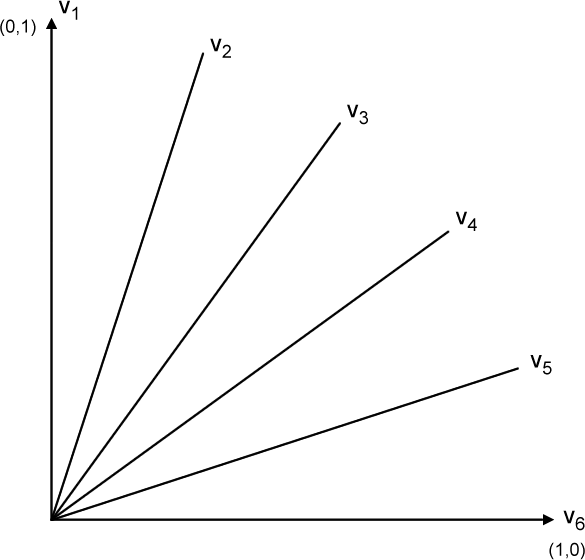
\includegraphics[width=0.5\textwidth]{cap_otimizacao-multi/figs/moead-ex1}
	\caption{\label{fig_moead_ex1}Exemplo de aplicação do MOEA/D: geração dos vetores de peso}
\end{figure}

\begin{figure}[!htbp]
	\centering
	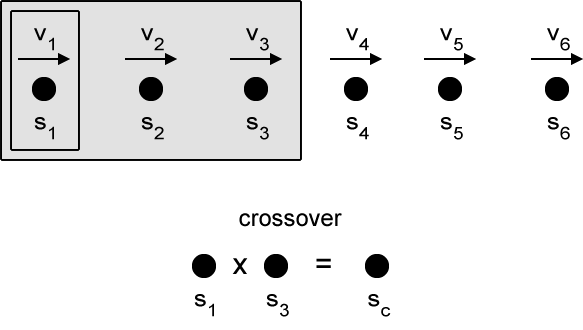
\includegraphics[width=0.5\textwidth]{cap_otimizacao-multi/figs/moead-ex2}
	\caption{\label{fig_moead_ex2}Exemplo de aplicação do MOEA/D: geração de soluções}
\end{figure}

\begin{figure}[!htbp]
	\centering
	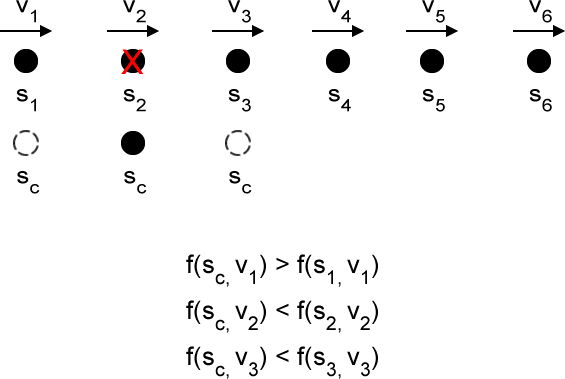
\includegraphics[width=0.5\textwidth]{cap_otimizacao-multi/figs/moead-ex3}
	\caption{\label{fig_moead_ex3}Exemplo de aplicação do MOEA/D: seleção de soluções}
\end{figure}

\begin{figure}[!htbp]
	\centering
	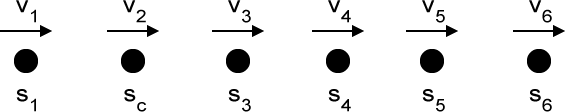
\includegraphics[width=0.5\textwidth]{cap_otimizacao-multi/figs/moead-ex4}
	\caption{\label{fig_moead_ex4}Exemplo de aplicação do MOEA/D: configuração da estrutura após a primeira iteração}
\end{figure}

\FloatBarrier
\subsection{NSGA-III}

O \textit{Non-dominated Sorting Genetic Algorithm III} (NSGA-III) \cite{Deb2014} é uma extensão do NSGA-II, elaborada com o objetivo de prover um melhor desempenho do \textit{framework} ao lidar com problemas de mais de três objetivos (\textit{many-objective}). Ele se diferencia da versão anterior principalmente na fase de reinserção ou seleção natural, onde, ao invés de usar a distância de aglomeração (\textit{crowding distance}) para diferenciar soluções em uma mesma fronteira, utiliza um método de agrupamento, no qual os indivíduos são divididos em nichos de acordo com suas proximidades em relação aos pontos de referência.

O NSGA-III é caracterizado pelo processo de atribuição de nicho chamado de classificação não-dominada baseada em pontos de referência. Sua ideia é traçar uma figura geométrica de uma dimensão a menos que o número de objetivos nos pontos extremos da primeira fronteira. Um número pré-definido de pontos de referência equidistantes são distribuídos ao longo da figura, cada qual representando um respectivo nicho.

Os pontos de referência nada mais são do que um conjunto de pontos no espaço de objetivos que busca guiar o processo de busca, melhorando tanto a diversidade quanto a convergência do conjunto de soluções do algoritmo. Esses pontos representam as regiões nas quais se deseja encontrar soluções não dominadas, direcionando a busca evolutiva. Os pontos de referência podem ser gerados a partir de uma abordagem estruturada ou previamente fornecidos ao algoritmo. Por exemplo, se o usuário tem preferências sobre as regiões do espaço de busca que devem ser exploradas. 

Na abordagem estruturada, é gerado um simplex unitário na dimensão imediatamente inferior à quantidade de objetivos. Por exemplo, se a quantidade de objetivos é 3, o simplex gerado tem dimensão 2. O simplex unitário é definido como a generalização do triângulo para uma determinada quantidade de dimensões. Assim, um simplex bi-dimensional é um triângulo, um simplex tridimensional é um tetraedro, e assim sucessivamente. O simplex gerado intercepta cada um dos eixos no ponto unitário, ou seja, para um simplex de dimensão 1 em um espaço de dois objetivos, os seus dois vértices são $v_1 = (1;0)$ e $v_2 = (0;1)$. Para cada eixo, são feitas $d$ subdivisões entre 0 e 1, onde $d$ é um parâmetro do NSGA-III.  Por exemplo, para 4 subdivisões $(d = 4)$, temos os pontos 0; 0,25; 0,5; 0,75 e 1 sobre cada eixo. Por exemplo, em um problema de 2 objetivos, pode-se definir uma estrutura similar à apresentada na \autoref{fig_nsga3}, para se estabelecer pontos de referência próximos aos quais se deseja encontrar soluções não dominadas, direcionando a busca evolutiva.

\begin{figure}[!htbp]
	\centering
	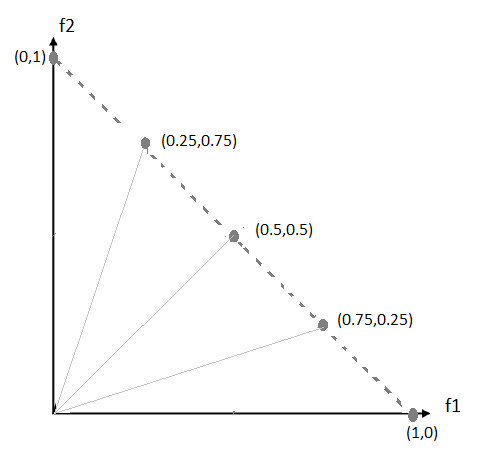
\includegraphics[width=0.5\textwidth]{cap_otimizacao-multi/figs/nsga3}
	\caption{\label{fig_nsga3}Pontos de referência para um problema com 2 objetivos (normalizados) e 4 subdivisões.}
\end{figure}

Para classificar uma solução da população corrente, encontra-se a reta mais próxima formada a partir dos pontos de referência. Ao final, são selecionadas (sobrevivem) as soluções localizados nas regiões menos lotadas do espaço de busca, com um menor número de indivíduos.

O NSGA-III segue os mesmos passos do NSGA-II até a classificação das soluções em fronteiras não dominadas, onde na primeira fronteira ($F_1$) estão contidas todas as soluções não dominadas da população, na segunda fronteira ($F_2$) estão as soluções que são dominadas apenas pela primeira fronteira, e assim por diante. A população para a próxima iteração é iniciada como um conjunto vazio ($P_{t+1} = \emptyset$), e então incluem-se as soluções de cada fronteira, começando pela primeira, até que se atinja o tamanho máximo da população $(tam\_pop)$. Se incluir a próxima fronteira faz com que o tamanho de $P_{t+1}$ atinja ou ultrapasse o valor $(tam\_pop)$, deve-se tomar uma de duas decisões em relação à inclusão dos indivíduos dessa fronteira ($F_{last}$):

\begin{enumerate}
	\item Se $|P_{t+1}| + |F_{last}| = tam\_pop$, faz-se $P_{t+1} = P_{t+1} \cup F_{last}$ e parte-se para a próxima iteração.
	\item Se $|P_{t+1}| + |F_{last}| > tam\_pop$, acrescentar os elementos de $F_{last}$ a $P_{t+1}$ ultrapassa o limite da população. Portanto, é necessário selecionar quais soluções de $F_{last}$ devem ser incluídas em $P_{t+1}$. No NSGA-III, essa seleção é realizada por meio da classificação não-dominada baseada em pontos de referência.
\end{enumerate}

O NSGA-III se difere do seu precursor (NSGA-II) justamente nesse processo de selecionar os indivíduos de $F_{last}$. O primeiro passo da classificação não-dominada baseada em pontos de referência é a definição de um conjunto de soluções referência ($S_r$). Geralmente, o conjunto escolhido é a primeira fronteira não dominada, ou seja, $F_1$. Isso só não acontece quando o número de soluções na primeira fronteira é menor que o número de objetivos ($m$) e existe outra fronteira com pelo menos $m$ elementos. Nesse caso, a primeira fronteira com $m$ ou mais elementos é escolhida ($F_{best}$). Se a fronteira escolhida foi $F_{last}$, então $S_r = F_{last}$, caso contrário, $S_r = F_{last} \cup F_{best}$.

O conjunto de soluções referências ($S_r$) é então normalizado. Os maiores valores em $S_r$ para cada objetivo se tornam 1, enquanto os menores se tornam 0. A seguir, calcula-se um ponto extremo para cada objetivo de acordo com as soluções em $F_{best}$. Para determiná-los, basta encontrar a solução em $F_{best}$ que mais se aproxima do eixo correspondente ao objetivo (distância euclidiana baseada no valor normalizado). Para isso, ao calcular a distância da solução $s$ ao eixo do objetivo, determina-se a distância entre $s$ e um ponto imaginário $p$ com todas as coordenadas valendo zero, exceto para o objetivo em questão, cujo valor é o mesmo de $s$. Por exemplo, para um problema de 6 objetivos, o cálculo da distância entre a solução $s = [0,8; 0,4; 0,5; 0,7; 0,1; 0,4]$ e o eixo do quarto objetivo é dada pela distância euclidiana entre $s$ e o ponto $p = [0; 0; 0; 0,7; 0; 0]$, que vale $\sqrt{0,8^2 + 0,4^2 + 0,5^2 + 0 + 0,1^2 + 0,4^2} = 1,22$.

O passo seguinte, é distribuir as soluções em $F_{last}$ em nichos. Os nichos são criados de acordo com os pontos extremos (um por objetivo) e o número de subdivisões ($d$, parâmetro do NSGA-III). Inicialmente, cria-se uma sequência de retas que ligam os pontos extremos uns aos outros. Para 6 objetivos, por exemplo, liga-se o primeiro ponto extremo aos outros 5, criando 5 retas. O segundo ponto é ligado a todos os outros com exceção do primeiro que já está ligado, formando mais 4 retas. Com o terceiro ponto extremo, criam-se mais 3 retas. Com o quarto ponto formam-se duas novas retas e a última reta é criada pelos pelos quinto e sexto pontos, gerando ao todo 15 retas. Em cada uma delas distribuem-se $d$ pontos igualmente espaçados chamados de pontos de referência ($P_{ref}$).

Com o conjunto de pontos de referência ($P_{ref}$) em mãos, basta associar um nicho (inicialmente vazio) a cada ponto e então distribuir as soluções em $F_{last}$. Para cada ponto $p \in F_{last}$, verifica-se a distância entre ele e todos os pontos de referência $r \in P_{ref}$. Em seguida, $p$ é incluído ao nicho referente ao ponto $r$ com a menor distância para $p$. Após distribuir todas soluções entre os nichos, ordena-se cada nicho de acordo com as distâncias da solução para o ponto de referência. A solução mais distante do ponto de referência deve estar na primeira posição do nicho e a mais próxima, na última.

Como todas as soluções de $F_{last}$ estão classificadas em nichos, basta adicionar uma por uma em $P_{t+1}$ até que o limite no tamanho da população ($tam\_pop$) seja atingido. Cada nicho possui um contador que inicia em 0. Cada vez que uma solução do nicho é escolhida, seu contador é incrementado em 1. Sempre, ao selecionar uma solução, escolhe-se o nicho com o menor valor de contador, e então extrai-se dele a solução na última posição (mais próxima do ponto de referência).

Com a população $P_{t+1}$ formada de exatamente $tam\_pop$ indivíduos, volta a se realizar o processo idêntico ao NSGA-II, até que novamente, na próxima iteração, após a geração dos filhos, seja necessário selecionar os indivíduos sobreviventes. Mais detalhes sobre o processo de agrupamento podem ser obtidos no artigo original do algoritmo \cite{Deb2014}.

\subsection{SPEA2-SDE}

O \textit{SPEA2 with Shift-Based Density Estimation} (SPEA2-SDE) \cite{Spea2SDE} é uma pequena alteração no algoritmo SPEA2 que possibilita lidar com problemas que envolvam 4 ou mais objetivos de uma forma muito mais eficiente. A única alteração está no cálculo de distância entre duas soluções. Suponha que $s_1$ e $s_2$ sejam dois indivíduos na população e que seus valores no espaço de objetivo sejam, respectivamente, $[5, 10, 351, 7, 15]$ e $[6, 8, 15, 9, 14]$. No SPEA2, a distância entre $s_1$ e $s_2$ é dada pela distância euclidiana dos dois vetores ($dist$), ou seja:

\begin{equation}dist(s_1, s_2) = \sqrt{(5-6)^2 + (10-8)^2 + (351-15)^2 + (7-9)^2 + (15-14)^2} = 336,0148\end{equation}

As duas soluções são bem próximas, pois só estão distantes em uma das 5 coordenadas. Entretanto, o cálculo de distância do SPEA2 não reflete isso, o que é prejudicial em problemas com muitos objetivos. A fim de resolver esse problema, \cite{Spea2SDE} introduziram o cálculo de distância \ac{SDE}, que nada mais faz do que transladar a coordenada mais distante do segundo ponto para o mesmo valor no primeiro ponto. Isto é, antes de calcular a distância euclidiana, identifica-se a coordenada que exibe maior diferença entre os dois pontos. No caso de $s_1$ e $s_2$, a terceira coordenada é a que possui esse comportamento. Em seguida, é realizada a translação do segundo ponto na coordenada identificada para que seja igual ao primeiro ponto, (no exemplo, $s_2' = [6, 8, \textbf{351}, 9, 14]$). A distância SDE é, então, determinada pela distância euclidiana entre o primeiro ponto ($s_1$) e o segundo ponto transladado ($s_2'$). No exemplo, a distância SDE obtida é: 

\begin{equation}dist_{SDE}(s_1, s_2') = \sqrt{(5-6)^2 + (10-8)^2 + (351-351)^2 + (7-9)^2 + (15-14)^2} = 3,1622\end{equation}

A distância SDE descarta a coordenada mais distante ao calcular as distâncias, permitindo assim que pontos distantes em apenas uma coordenada ainda sejam considerados próximos. Todo o restante do processo do SPEA2-SDE segue os mesmos passos do algoritmo original.

\subsection{MEAMT (AEMMT)}

O \textit{Multi-Objective Evolutionary Algorithm with Many Tables} (MEANDS) \cite{Brasil2013} foi proposto originalmente com o nome em português Algoritmo Evolutivo Multiobjetivo com Muitas Tabelas (AEMMT) e será referenciado como tal no decorrer desta dissertação. Assim como o MOEA/D, o AEMMT decompõe o problema multiobjetivo em subproblemas menores de um único objetivo. Entretanto, o AEMMT utiliza um esquema de tabelas, onde cada tabela representa uma combinação diferente dos objetivos investigados. A função que transforma os múltiplos objetivos em um valor escalar é a média aritmética e cada tabela mantém os melhores indivíduos, considerando o valor médio dos objetivos que ela representa. A cada geração, duas tabelas são selecionadas para o cruzamento. Dois pais, um de cada tabela, são sorteados aleatoriamente para gerarem um único filho. Essa nova solução (filho) é avaliada em todas as tabelas, entrando naquelas em que representar uma melhor aptidão em relação aos indivíduos atuais. Naturalmente, como um único \textit{crossover} é realizado e um único filho é gerado a cada iteração, o AEMMT precisa de mais gerações para alcançar o mesmo número de soluções avaliadas que os algoritmos citados anteriormente.

A quantidade de tabelas é determinada pelo número de combinações possíveis entre os objetivos. Para quatro objetivos ($f_1, f_2, f_3, f_4$), por exemplo, serão criadas 15 tabelas de combinações mais uma tabela extra, usada para guardar os indivíduos não-dominados, como ilustrado na \autoref{fig_aemmt_tabelas}. Cada tabela possui um limite máximo de indivíduos. No início do algoritmo, gera-se um número pré-definido de soluções aleatórias de forma a preencher todas as tabelas com soluções diferenciadas umas das outras. Por exemplo, nos experimentos com o PRM descritos no Capítulo 6, foi gerado um número de soluções equivalente à quantidade de tabelas criadas multiplicada pelo tamanho máximo das tabelas (30). Assim, no caso do PRM com 4 objetivos, foram criadas $16 \times 30 = 480$ soluções e extraídas as 30 melhores para cada tabela, de acordo com a combinação de objetivos de cada uma.

No laço principal, um indivíduo só entra em uma tabela $t$, se for melhor que a pior solução na população atual de $t$. Com relação à tabela de dominância, sempre que um filho é gerado e ele não é dominado por nenhum outro indivíduo da tabela, ele é incluído. A restrição no tamanho da tabela de dominância pode ser diferente das demais e, sempre que o limite for atingido, é feito um truncamento priorizando a permanência das soluções com maior valor de média aritmética entre todos os objetivos.

\begin{figure}[!htbp]
	\centering
	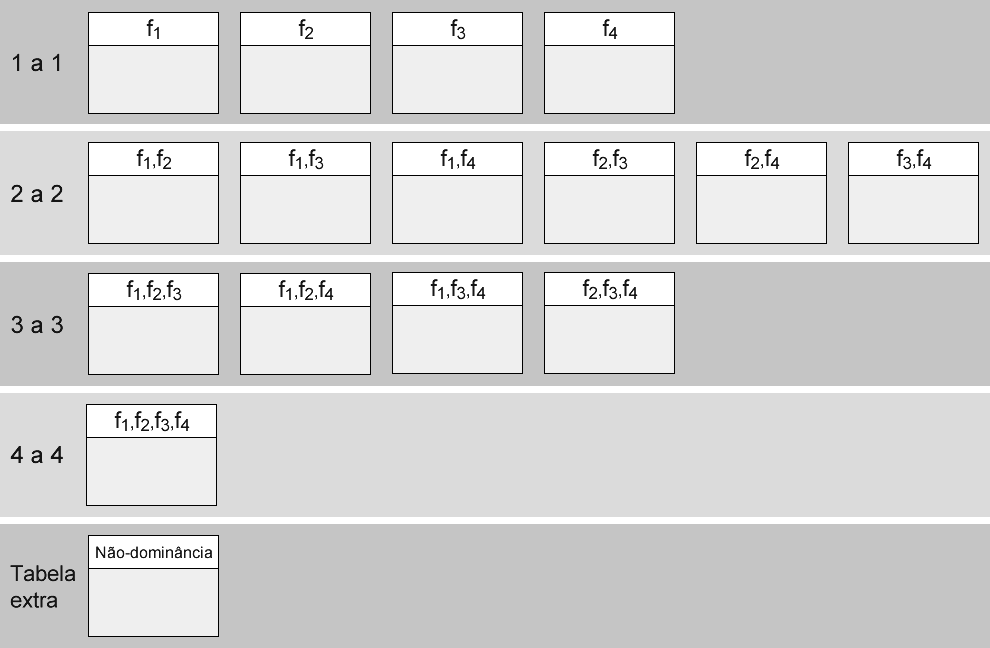
\includegraphics[width=1\textwidth]{cap_otimizacao-multi/figs/aeemt-tabelas}
	\caption{\label{fig_aemmt_tabelas}Exemplo da quantidade de tabelas usadas pelo AEMMT}
\end{figure}

Após a geração e preenchimento das tabelas, inicia-se o laço principal. A cada iteração são escolhidas duas tabelas via torneio duplo, de acordo com suas pontuações. A pontuação de uma tabela tem valor inicial zero e sempre que essa tabela gera um filho que sobrevive para a geração seguinte, sua pontuação é incrementada. De acordo com as observações dos autores da pesquisa, após um determinado número de gerações, as pontuações das tabelas eram tais que sempre as mesmas eram escolhidas para o \textit{crossover}, assim, na versão final do algoritmo, as pontuações são zeradas a cada 100 gerações. Considerando-se as duas tabelas selecionadas, sorteia-se um indivíduo de cada e efetua-se o cruzamento entre eles. O filho gerado é, então, comparado tabela a tabela, sendo incluído naquelas em que representar uma melhoria, ou seja, o novo indivíduo supera pelo menos o pior indivíduo da tabela corrente. Após a execução de todas as gerações, dá-se como resultado o conjunto não dominado, considerando-se as soluções de todas as tabelas.

\subsection{MEANDS (AEMMD)}
\label{section_aemmd}

O \textit{Multi-Objective Evolutionary Algorithm based on Non-dominated Decomposed Sets} (MEAMT) \cite{Lafeta2016} foi proposto originalmente com o nome em português Algoritmo Evolutivo Multiobjetivo com Múltiplas Dominâncias (AEMMD) e será referenciado como tal no decorrer desta dissertação. O AEMMD é uma modificação do AEMMT que, apesar de usar o mesmo processo de divisão do problema multiobjetivo, abandona a ideia de escalarização e adota o conceito de dominância também usado nos métodos clássicos (e.g. NSGA-II e SPEA2). No AEMMD, ao invés de se utilizar a média dos objetivos da tabela para avaliar o indivíduo, lança-se mão da relação de dominância de Pareto. Como o conceito de tabela do AEMMT e dos métodos que o inspiraram remete ao conceito de média e ordenação, essa estrutura, no AEMMD, é chamada apenas de conjunto de não-dominância. Um indivíduo novo $s$ só entra no conjunto $C_{nd}$, se $s$ não for dominado por nenhuma solução em $C_{nd}$ (considerando apenas os objetivos de $C_{nd}$). Além disso, se $s$ entra em $C_{nd}$, todas as soluções em $C_{nd}$ dominadas por $s$ são removidas.

O primeiro passo do AEMMD é gerar a lista de conjuntos de não-dominância, considerando todas as combinações de objetivos possíveis a partir de dois a dois. Combinações de um único objetivo não são criadas, pois o conceito de dominância é válido a partir de dois valores. Diferentemente do AEMMT, os conjuntos não possuem limite de tamanho e podem crescer indefinidamente. Por exemplo, para um problema de quatro objetivos ($f_1, f_2, f_3, f_4$), 11 conjuntos seriam gerados, como pode ser observado na Figura \ref{fig_aemmd_tabelas}.

\begin{figure}[!htbp]
	\label{fig_aemmd_tabelas}
	\centering
	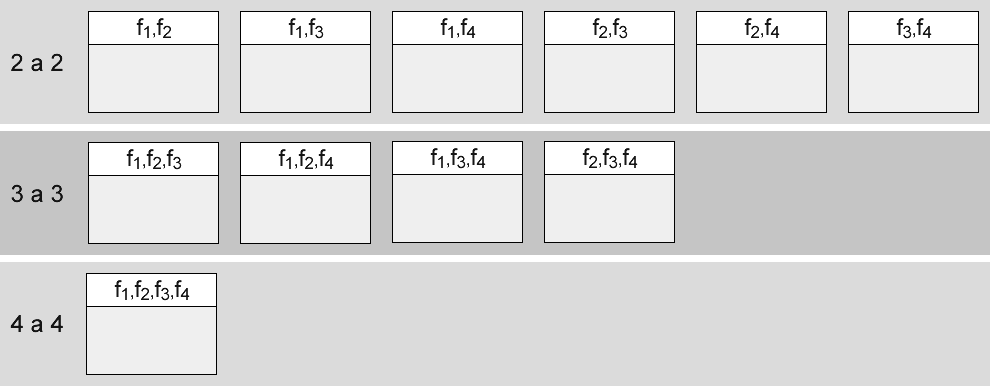
\includegraphics[width=1\textwidth]{cap_otimizacao-multi/figs/aeemd-tabelas}
	\caption{Exemplo da quantidade de conjuntos usados pelo AEMMD}
\end{figure}

Com os conjunto de não-dominância criados, gera-se um número pré-definido de soluções aleatórias, distribuindo-as pelos conjuntos de acordo com a relação de dominância de Pareto. Assim como no AEMMT, a cada iteração do algoritmo, é utilizado um torneio duplo para selecionar dois conjuntos de acordo com suas pontuações. Entretanto, a pontuação dos conjuntos no AEMMD é diferente da pontuação nas tabelas do AEMMT. Ao invés de conceder um ponto sempre que o conjunto contribui com um pai que gera um indivíduo sobrevivente, pontua-se quando ele recebe um indivíduo novo. Uma vez selecionados os dois conjuntos, sorteia-se um representante de cada e gera-se um único filho, o qual é comparado conjunto a conjunto, sendo inserido naqueles onde representa uma solução não dominada. Outra diferença observada pelo autor em relação ao AEMMT é que o novo modelo de pontuação não degrada no decorrer das gerações, ou seja, mesmo após várias gerações, ainda existe grande diversidade na escolha dos conjuntos pais, tornando desnecessária a reinicialização das pontuações associadas aos conjuntos \cite{Lafeta2016}. Espera-se que ao final das gerações, a população do conjunto que considera todos os objetivos no seu critério de dominância tenha convergido para a fronteira de Pareto. 

\section{Algoritmos multiobjetivos baseados em colônias de formigas}

A maior parte dos métodos de busca multiobjetivo são baseados em algoritmos genéticos. Entretanto, uma alternativa que ainda é pouco explorada são as técnicas inspiradas em inteligência coletiva. Dentre elas, optou-se por investigar métodos de otimização baseados em colônias de formigas, os quais são particularmente adequados para lidar com problemas discretos, como aqueles utilizados neste trabalho (problema da mochila multiobjetivo e problema do roteamento multicast). Dentre os ACOs multiobjetivos encontrados na literatura, destacam-se o MOACS \cite{Baran2003} e o MOEA/D-ACO \cite{Ke2013}.

\subsection{MOACS}

O \textit{Multi-Objective Ant Colony Optimization Algorithm} (MOACS) \cite{Baran2003} é uma adaptação do ACO original que torna possível a otimização de múltiplos objetivos utilizando uma única estrutura de feromônios, múltiplas heurísticas e um arquivo de soluções não dominadas. Esse algoritmo foi proposto originalmente para o problema de roteamento de veículos com janelas de tempo e, posteriormente, foi aplicado no problema do roteamento multicast \cite{Pinto2005}. Uma variação desse algoritmo, mais voltada à solução de problemas \textit{many-objective}, foi apresentada em \cite{Riveros2016}, a qual é utilizada neste trabalho. A diferença básica entre a modificação de Riveros e o modelo original está na geração dos pesos para as heurísticas. No modelo original, são geradas todas as combinações possíveis, o que é inviável em problemas com muitos objetivos. Na versão \textit{many-objective}, o problema é solucionado através de uma amostragem desses vetores de peso. O funcionamento básico do MOACS é descrito no Algoritmo \ref{alg_moacs}.

\begin{algorithm}
	\caption{Algoritmo MOACS}
	\label{alg_moacs}
	\begin{algorithmic}[1]
		\State Inicialize a estrutura de feromônios $\tau_{ij}$ com $\tau_0$ /* $\tau_{0}$ é o valor inicial */
		\State Crie um conjunto vazio de soluções não-dominadas $ND$
		\While {Número máximo de iterações não for atingido}
		\For {$i \gets 0$ até $tamanho\_populacao$}
		\State Sorteie valores no intervalo $[0, w_{max}[$ para formar um vetor de pesos $W$ com $|H|$ posições
		\State Construa uma solução de acordo com a tabela de feromônios $\tau_{ij}$, as heurísticas ($H$) e os pesos $W$
		\State Atualize $ND$ com a nova solução
		\EndFor
		\If {$ND$ foi modificado}
		\State Reinicie a estrutura de feromônios fazendo $\tau_{ij} = \tau_0 \forall(i,j)$
		\Else
		\State Atualize a estrutura de feromônios com todas as soluções em $ND$
		\EndIf
		\EndWhile
		\State \Return $ND$
	\end{algorithmic}
\end{algorithm}

O processo de construção de uma solução depende do problema investigado. No MOACS, os principais componentes utilizados nesse processo são:

\begin{itemize}  
	\item Feromônios ($\tau_{ij}$): estrutura que guarda a quantidade de feromônios em cada partícula que pode formar a solução. No caso de problemas em grafos, representa a quantidade da substância em cada uma das arestas, indicando a frequência de suas utilizações;
	\item Heurísticas ($H$): conjunto de funções que estimam a qualidade de uma dada partícula que pode formar a solução. No caso de problemas em grafos, representa os vários pesos em uma aresta. Por exemplo, num grafo que representa uma rede de computadores com informações de custo, distância e tráfego, $H$ poderia ser formado de três funções que recebem uma aresta $(i,j)$ e devolvem, respectivamente, os valores de suas métricas custo, distância e tráfego.
	\item Peso máximo de uma heurística ($w_{max}$): representa a granularidade da escala de pesos que cada heurística pode assumir. Em \cite{Riveros2016}, propõe-se $w_{max} = 3$, de forma que cada função possa ser classificada como 0 (não importante), 1 (importante), 2 (muito importante).
	\item Vetor de pesos ($W$): O vetor de pesos atribui a importância de cada heurística e normalmente é gerado de forma aleatória em cada iteração. Cada função de heurística recebe um valor inteiro representando o peso e variando no intervalo $[0, w_{max}[$.
\end{itemize}

Ao construir uma solução, utiliza-se o mesmo processo de decisão do ACO original, explicado na seção \ref{section_construcao_solucao}. A única diferença é que as múltiplas heurísticas do MOACS ($H$) são unificadas em uma única função $h(x)$, por meio de uma média ponderada. Nesse processo, utiliza-se o vetor de pesos $W$ para definir o fator de ponderação de cada heurística. Dessa forma, a função h(x) é dada por:

\begin{equation}h(x) = \frac{\sum_{i \gets 0}^{size(H)}\ H_i(x) \times W_i}{\sum_{w \in W} w}\end{equation}

Em cada época (iteração do ACO), atualiza-se o arquivo de soluções não dominadas com as novas soluções geradas. Se o arquivo foi atualizado após a criação de todas as soluções, reiniciam-se as informações de feromônio, redefinindo todos os valores na estrutura $\tau_{ij}$ para o valor inicial de feromônio $\tau_0$. Caso o arquivo tenha se mantido estável, ou seja, nenhuma das novas soluções é não-dominada, atualizam-se as quantidades de feromônio na estrutura de acordo com as soluções no arquivo.

Considerando-se um problema em grafos, para atualizar a estrutura $\tau_{ij}$ com uma solução $s$, faz-se:

\begin{equation}\tau_{ij} = (1 - \rho) \times \tau_{ij} + \rho \times \Delta\tau(s) \qquad \forall(i,j) \in s\end{equation}

Sendo:
\begin{itemize} 
	\item $\rho$: coeficiente de evaporação;
	\item $\Delta\tau(s)$: Quantidade de feromônios depositados pela solução $s$, que por sua vez é definida por:
\end{itemize}

\begin{equation}\Delta\tau(s) = \frac{1}{performance(s)}\end{equation}

Na fórmula anterior, $performance(s)$ é dado pela soma dos valores de $s$ no espaço de objetivos. Neste caso, considera-se um problema de minimização. Por exemplo, se os objetivos são reduzir o custo, o tráfego e o atraso (\textit{delay}) de uma rede, então, $performance(s) = custo(s) + trafego(s) + delay(s)$. Para problemas de maximização, basta inverter a equação.

Após todas as iterações do MOACS, espera-se obter no arquivo uma boa aproximação da fronteira de Pareto. 

\subsection{MOEA/D-ACO}
O \textit{Multiobjective evolutionary algorithm based on decomposition ACO} (MOEA/D-ACO) \cite{Ke2013} é um método que adapta o algoritmo MOEA/D (seção \ref{section_moead}) ao \textit{framework} de otimização por colônia de formigas (ACO). Os conceitos de células e vizinhanças são reutilizados, enquanto que a reprodução local, inexistente no ACO, é substituída por um processo de construção da solução levemente modificado. Além disso esse método introduz um novo conceito de grupos que é utilizado para agrupar as formigas de acordo com seus vetores de peso. Nesse algoritmo, o termo formiga corresponde ao conceito de célula do MOEA/D.

O primeiro passo do MOEA/D-ACO consiste em gerar os vetores de peso que, assim como no MOEA/D, são arranjos de valores entre 0 e 1, cujas somas valem 1. A geração pode ser aleatória ou seguir alguma distribuição pré-definida. No caso deste trabalho, utilizou-se a distribuição uniforme proposta no artigo original \cite{Ke2013}. Atribui-se cada vetor a uma formiga e cria-se a estrutura de vizinhanças, onde cada formiga é associada a uma vizinhança contendo as $v_{size}$ formigas mais próximas de acordo com os vetores de peso (incluindo ela mesma). O segundo passo do algoritmo determina os grupos, sendo que cada grupo recebe um novo vetor de pesos gerado da mesma maneira que os pesos anteriores. As formigas são então distribuídas entre os grupos de acordo com a proximidade entre seu vetor de pesos e o vetor de pesos do grupo (\textit{agrupamento}).

Com respeito às duas principais estruturas de um ACO, heurística e feromônios, cada formiga possui uma função heurística e cada grupo mantém uma estrutura de feromônios. Quando os grupos são criados, cada um recebe uma estrutura de feromônios com o valor máximo de feromônio em cada uma das posições. Por sua vez, quando a formiga é criada, recebe uma função heurística baseada na combinação de todas as funções heurísticas do problema e no vetor de pesos da própria formiga. O cálculo específico da heurística depende do problema.

O processo iterativo (evolução) do MOEA/D-ACO consiste em gerar as soluções, atualizar o conjunto de soluções não-dominadas $ND$, distribuir as novas soluções entre as formigas e atualizar as estruturas de feromônio. Primeiramente, para cada grupo $G$, geram-se as soluções para cada formiga $f \in G$. A solução é gerada com base nos feromônios de $G$, na heurística de $f$ e na solução atual de $f$. Tendo gerado todas as soluções para um grupo, atualiza-se o arquivo de soluções não-dominadas $ND$. Para cada nova solução $S$ que entrou no arquivo, modifica-se a estrutura de feromônios $\tau$ de $G$. Assim, o cálculo do feromônio de uma partícula $e$ na iteração $i+1$ ($\tau_{i+1}(e)$) é obtido a partir do seu feromônio atual ($\tau_i(e)$), como segue:

\begin{equation}
\tau_{i+1}(e)= 
\begin{cases}
\rho \times \tau_i(e) + \delta,& \text{se } e \in S\\
\rho \times \tau_i(e),              & \text{caso contrário}
\end{cases}
\end{equation}

\vspace{4mm} %4mm vertical space

Onde $e$ é uma possível partícula de uma solução para o problema investigado (qualquer aresta, no caso do PRM, ou item, para o PMM) da tabela de feromônios; $\rho$ é a taxa de evaporação; e $\delta$ é dado pelo inverso da soma dos valores da função de escalarização aplicada sobre cada solução não dominada de $G$ em relação ao vetor de pesos de $G$.

\begin{equation}\delta = \frac{1}{\sum_{s \in S_{nd}f_{esc}(s, W)}}\end{equation}
	
Sendo, $S_{nd}$ o conjunto de soluções não dominadas de $G$, $f_{esc}$ a função de escalarização, e $W$ o vetor pesos de $G$. Caso o problema seja de maximização, $\delta$ seria a soma dos valores, ao invés do inverso dela. 

Cada formiga armazena duas soluções, a solução atual, que de início é nula, e a nova solução, criada em cada iteração do algoritmo. Após a geração de novas soluções a atualização de feromônios para todos os grupos e suas formigas, deve-se decidir a solução atual de cada formiga com base nas novas soluções da vizinhança. Nesse processo, para cada formiga $f$ analisam-se as novas soluções presentes na vizinhança de $f$. Se alguma nova solução $sn$, que ainda não substituiu nenhuma outra, possui um \textit{fitness} melhor que o da solução corrente de $f_{esc}$ ($sc$), substitui-se $sc$ por $sn$. O \textit{fitness} é calculado de acordo com a média ponderada dos valores da solução em cada objetivo baseadas no vetor de pesos da formiga em questão. Neste trabalho, utilizou-se a soma ponderada como função \textit{escalarizadora}, mas qualquer uma das funções propostas em \cite{Zhang2007} pode ser usada.

O processo de construção da solução depende do problema investigado. Entretanto, o MOEA/D-ACO inclui duas novas características no processo, independente do problema. São elas:

\begin{itemize}
	\item \textbf{Influência da solução atual:} no MOEA/D-ACO, cada formiga mantém uma solução atual que influencia a construção da próxima solução com base em um parâmetro $\delta$. Isso acontece devido à introdução de um novo termo no cálculo de feromônio na construção da solução. Ao calcular a probabilidade de uma partícula $p$ (aresta ou item) fazer parte da solução, ao invés de adotar $feromonio(p)^\alpha$, considera-se $(\delta * x + feromonio(p))^\alpha$, sendo $x = 1$ se $p$ pertence à solução atual e $x = 0$ caso contrário.
	\item \textbf{Taxa de elitismo:} a maioria dos ACOs utilizam uma espécie de roleta para decidir qual partícula fará parte da solução. Aquelas com maior probabilidade têm maior chance de serem escolhidas, mas não necessariamente serão. Em uma estratégia elitista, não se utiliza a roleta. A partícula escolhida será aquela que receber o maior valor de probabilidade. No MOEA/D-ACO, utiliza-se uma taxa de elitismo que estipula a chance de uma partícula ser escolhida por elitismo ao invés de roleta.
\end{itemize}

O processo iterativo do algoritmo é executado até que uma condição de parada pré-definida seja atingida. Normalmente, adota-se um número máximo de iterações. Espera-se que, nesse momento, as soluções no conjunto $ND$ tenham convergido para a fronteira de Pareto.

\section{Outros algoritmos multiobjetivos}
Outros algoritmos multiobjetivos mais citados na literatura, mas que não foram analisados neste trabalho, são mencionados a seguir.

\textit{Vector Evaluated Genetic Algorithm} (VEGA) \cite{Schaffer1985} e \ac{MOGA} \cite{MOGA} foram os primeiros algoritmos multiobjetivos a aparecerem na literatura. Posteriormente, os algoritmos \ac{NSGA} \cite{Srinivas1994} e \ac{SPEA} \cite{Zitzler1999} foram propostos e são considerados os mais eficientes da primeira geração de \acp{AEMO}. A segunda geração de \acp{AEMO} é caracterizada por métodos elitistas, sendo que NSGA-II e o SPEA2 apresentados na \ref{section_bioinspired_algorithms} são considerados os mais eficientes dessa geração e até hoje são os mais utilizados na literatura, especialmente com 2 e 3 objetivos. Em problemas \textit{many-objective}, uma das principais dificuldades encontradas é o excesso de soluções não-dominadas, o que dificulta a identificação de melhores indivíduos e prejudica a convergência. Para lidar com esse problema, \citeonline{Aguirre2009} apresentam um conceito menos rigoroso de dominância, dando origem ao algoritmo $\epsilon$-MOEA. Por sua vez, a fim de reclassificar as soluções não dominadas e resolver o mesmo problema, \citeonline{Beume2007} propõem o algoritmo SMS-EMOA, no qual a evolução da população ocorre de acordo com indicadores de qualidade do conjunto de soluções. Nesse algoritmo, os autores usam o hiper-volume para avaliar soluções consideradas igualmente boas pela dominância de Pareto. \citeonline{Bader2011} utilizam uma ideia parecida ao propor o algoritmo Hype. Esse algoritmo também utiliza o hiper-volume como parâmetro para guiar a evolução da população. 

Em relação aos algoritmos de inteligência coletiva, o algoritmo MOEA/D-BACO foi proposto por \citeonline{SouzaPozo2015} e aplica uma variação do MOEA/D-ACO no \ac{UBQP}. Como para o UBQP as estruturas de feromônio crescem de forma exponencial em relação ao tamanho da entrada, o método MOEA/D-ACO original se torna inviável. A variação proposta pelos autores, algoritmo MOEA/D-BACO, visa solucionar esse problema através da substituição do ACO, no MOEA/D-ACO, pelo \ac{BACO} \cite{baco2006}, que é um algoritmo mais simples e promete menor tempo de execução em relação ao algoritmo original. Em 2001, Iredi, Merkle e Middendorf propuseram o algoritmo \textit{Bi-Criterion Optimization with Multi Colony Ant Algorithms} para o problema \ac{SMTTP} com dois objetivos \cite{BiCriterionAnt}. O algoritmo usa duas tabelas de feromônios (uma para cada objetivo) e cada formiga recebe dois valores de peso que são distribuídos uniformemente entre a colônia, esses valores representam o peso de cada objetivo nas decisões da formiga. A atualização dos feromônios é realizada com base nas formigas que geraram soluções não dominadas na geração corrente. \citeonline{BiCriterionAnt} também propõem um método com múltiplas colônias, onde cada colônia trabalha com duas tabelas de feromônios, mas, através da atribuição de pesos aos objetivos, pesquisam em regiões diferentes do espaço de busca. Segundo \citeonline{Ibanez2012}, os algoritmos os algoritmos \acp{MACO} seguem todos uma mesma formulação e que podem ser modelados como um único \textit{framework}, diferenciando apenas em algumas decisões de projeto, que seriam parâmetros desse \textit{framework} geral capaz de gerar qualquer MACO. Nesse trabalho, os autores classificam diversos MACOs na literatura e destacam onde se diferem, mostrando as estratégias que podem ser adotadas ao elaborar um algoritmo ACO multiobjetivo. Além disso, o artigo propõe uma forma de gerar automaticamente os parâmetros de um MACO a fim de obter os melhores valores possíveis para um determinado problema sem que se seja necessário testar manualmente diversas configurações.